%%%%%%%%%%%%%%%%%%%%%%%%%%%%%%%%%%%%%%%%%%%%%%%%%%%%%%%%%%%%%%%%%%%%%%%%%%%%%%%%
%2345678901234567890123456789012345678901234567890123456789012345678901234567890
%        1         2         3         4         5         6         7         8

\documentclass[letterpaper, 10 pt, conference]{ieeeconf}  % Comment this line out if you need a4paper

%\documentclass[a4paper, 10pt, conference]{ieeeconf}      % Use this line for a4 paper

\IEEEoverridecommandlockouts                              % This command is only needed if 
                                                          % you want to use the \thanks command

\overrideIEEEmargins                                      % Needed to meet printer requirements.

%In case you encounter the following error:
%Error 1010 The PDF file may be corrupt (unable to open PDF file) OR
%Error 1000 An error occurred while parsing a contents stream. Unable to analyze the PDF file.
%This is a known problem with pdfLaTeX conversion filter. The file cannot be opened with acrobat reader
%Please use one of the alternatives below to circumvent this error by uncommenting one or the other
%\pdfobjcompresslevel=0
%\pdfminorversion=4

% See the \addtolength command later in the file to balance the column lengths
% on the last page of the document

% The following packages can be found on http:\\www.ctan.org
\usepackage{graphicx} % for pdf, bitmapped graphics files
\usepackage{epsfig} % for postscript graphics files
\usepackage{mathptmx} % assumes new font selection scheme installed
\usepackage{times} % assumes new font selection scheme installed
\usepackage{amsmath} % assumes amsmath package installed
\usepackage{amssymb}  % assumes amsmath package installed

\title{\LARGE \bf
From Evaluating to Teaching:\\
Rewards and Challenges of Human Control for Learning Robots
}


\author{Emmanuel Senft$^{1}$, S\'{e}verin Lemaignan$^{2}$, Paul Baxter$^{3}$ and Tony Belpaeme$^{1,4}$% <-this % stops a space
\thanks{*This work was supported by the EU FP7 DREAM project (grant no.  611391).}% <-this % stops a space
\thanks{$^{1}$ University of Plymouth, CRNS, Plymouth, UK\newline
        {\tt\small emmanuel.senft@plymouth.ac.uk}}%
\thanks{$^{2}$ University of the West of England, BRL, Bristol, UK}%
\thanks{$^{3}$ University of Lincoln, L-CAS, Lincoln, UK}%
\thanks{$^{4}$ Ghent University, IDLab—imec, Ghent, Belgium}%
}

\begin{document}

\maketitle
\thispagestyle{empty}
\pagestyle{empty}


%%%%%%%%%%%%%%%%%%%%%%%%%%%%%%%%%%%%%%%%%%%%%%%%%%%%%%%%%%%%%%%%%%%%%%%%%%%%%%%%
\begin{abstract}
Keeping a human in a robot learning loop can provide many advantages to improve the learning process. However, most of these improvements are only available when the human teacher is in complete control of the robot's behaviour, and not when only providing feedback.
This human control can make the learning process safer, allowing the robot to learn in high-stakes scenarios such as social interaction. It also allows faster learning as the human guides the robot to the relevant part of the state and can provide additional information to the learner. Learning from end users also improves the precision of the final policy as it can be specifically tailored to any situations. Furthermore, additional information from the teacher enables the learning algorithms to learn for wider world representations, increase the generalisability of a deployed system. %PB: learning from end users will provide domain specific/specialist knowledge - I'm not sure about generalisation and precision of the policy (unless you provide more detail...) ES: a human can guide more efficiently a robot leading to a policy specifically adapted to each scenario + this guidance allow to learn from more general representations of the world, with could allow a same system to learn multiple task/different behaviour from a single implementation PB: sounds like two separate arguments. First point, yes, a specific policy for each scenario. Second point seems to refer to the generalisability of the system before training?
%ES: yes, it's true it's unclear, generalisability as it could learn to complete different task, and precision, policies can be specifically tailored to each task.
%PB: worth splitting this into two separate sentences then
Finally, this progressive teaching might create trust between the learner and the teacher, easing the deployment of the autonomous robot. %PB: not sure how trust comes into this, unless you can suggest a causal relationship - why would they trust a progressive learning of the robot? Could be argued that the reverse is true...
%ES: by observing the robot learning and hopefully improving its behaviour, a teacher can have a more precise model of the robot's behaviour which might, if the learning work, create trust in the agent to make correct decisions, potentially leading to an easier deployment
%PB: how about trust would build/be maintained if the performance/efficacy of the robot behaviour remains high from the start, rather than gradually builds. The progressive teaching of SPARC ensures this...?
%ES: There are 2 types of performance: the executed behaviour: always high with SPARC and the policy of the robot which generally starts from 0 and progressively develops until reaching a efficient one - maybe the trust is unclear, it's between the teacher and the robot, not the user and the robot
%PB: ok, that bit should be clarified then... howevr, is trust a concept you actually investigated? I thought it was more perception of performance/workload? argument could be made that the two are linked - is that what you wish to do here?
%ES: in the last study, we have report of the teacher stating that she starts trusting the robot more and so on, so it's not only about performance but also about how to experience the robot policy might make it easier to trust it, compared to something developed offline from demonstrations and directly thrown in the world without supervision or validation phase
%PB: in that case, keep as is!
%However, such control comes with challenges: the interface (GUI) needs to be complex to handle rich communication between the learner and the teacher. It also needs to include the teacher in the action loops with time constraints, and expose the robot to human errors too. %PB: you mean that while the teacher is observing the robot's errors, the robot also learns from any potential teacher's errors? ES: or if not learning, being able to deal with them - for example discarding erroneous demonstrations PB: do you think this is a bit of a subtle point for the abstract? worth mentioning in the discussion for example, but perhaps not here...
%ES: true, it depends of the way its implemented also. I intended to have a bit of all the points already present in the abstract, but it might be a bit confusing
%PB: bear with me here... ES: sounds good so far
However, with such control comes a range of challenges. Firstly, the rich communication between the robot and teacher needs to be handled by an interface, which could become complex. Secondly, the teacher needs to be embedded within the robot action cycle, imposing time constraints, which increases the complexity of the requirements on the teacher. Finally, given a cycle of interaction between the robot and teacher, any mistakes made by the teacher will be propagated to the robot, thus introducing a complicating factor to the learning process.
%PB: that's an alternative attempt, some bits need cleaning up: does this do what you need it to?
%ES: Yes, it's much clearer, I'll see in a bit how to combine everything together
Nevertheless, we are convinced that empowering the robot teacher with ways to control a robot's behaviour has the potential to drastically improve both the learning process (allowing robots to learn in a wider range of environments) and the experience of the teacher. %PB: and performance of the robot and/or experience of the teacher?
%ES: True: during the teaching and after

\end{abstract}


%%%%%%%%%%%%%%%%%%%%%%%%%%%%%%%%%%%%%%%%%%%%%%%%%%%%%%%%%%%%%%%%%%%%%%%%%%%%%%%%
\section{INTRODUCTION}

Interactive Machine Learning (IML) \cite{fails2003interactive,amershi2014power} differs from Classical Machine Learning (CML) in the fact that the learning process is not one single monolithic step leading to a static classifier or robot behaviour, but a continuous iterative improvement of the behaviour. IML relies on a series of small learning steps progressively leading to a complete and autonomous system. Additionally, IML makes use of humans in the learning loop, to direct the learning process, making it at the same time faster, more adequate to the task and more efficient.

IML can take two forms: human supported classifiers (closer to semi-supervised learning) or agent learning to interact from human guidance (supervised reinforcement learning). A classical example of the first category is Active Learning, a learning process giving to the learner the opportunity to take a more active stance in the process, asking questions and querying labels from an oracle, often a human being \cite{settles2012active}. The second category relates to agents learning to interact in an environment and profiting from humans inputs to improve the learning process. In this case, the learner is not in control of the datapoints it has to classify as those come directly form the environment; in fact, the agent interact in an environment reacting to its actions and requires a policy leading to a successful outcome in the task. The human can provide additional information to support the agent in developing its policy.

This work is focused on the second category, agents learning from human supervision to interact in an environment. An example is presented in Figure \ref{fig:frame}, where a robot is taught to interact with a child, supporting them in an educational activity. Compared to CML, IML holds the promises of faster and more flexible learning leading to a policy more adapted to current task \cite{fails2003interactive,amershi2014power}.

\begin{figure}[ht]
	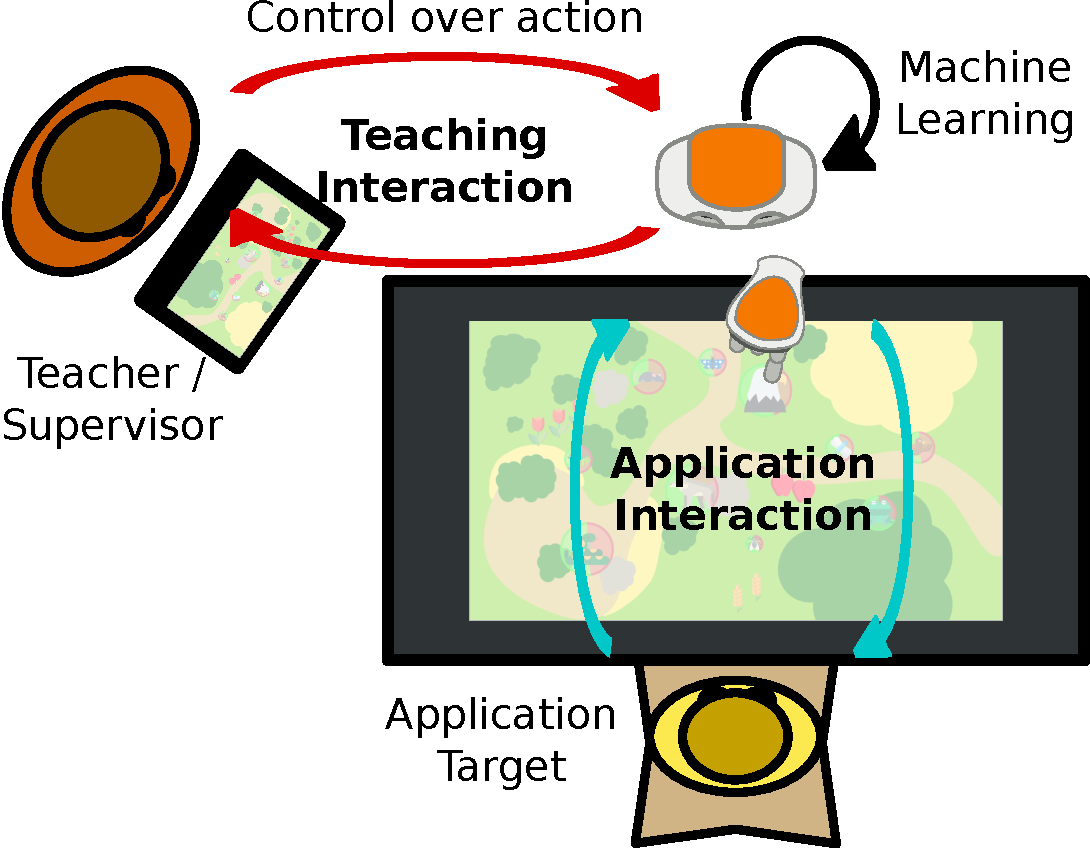
\includegraphics[width=.8\linewidth]{setup.pdf}
	\centering
	\caption{Example of a human teaching a robot to interact with a child in an educational scenario.}
	\label{fig:frame}
\end{figure}

In the context of agents learning to interact, a classical approach is to use a human to provide rewards on the robot's behaviour \cite{knox2009interactively}. The scenario is similar to Reinforcement Learning (RL) \cite{sutton1998reinforcement}, where an agent interacts in an environment providing rewards and where the agent has to maximise a notion a cumulative reward. Compared to traditional RL, using humans to distribute rewards possesses many advantages: no explicit reward function has to be provided, the human can anticipate the impacts of actions, reducing the challenge of credit assignment, and finally, the teachers can scaffold they reward distribution to help the agent to progressively improve its action policy \cite{macglashan2017interactive}. This way to support agent learning is attractive as it already provides advantages compared to classic RL and requires a simple interface between the teacher and a robot: the teacher needs to be able to observe the robot's behaviour and only provide a scalar evaluation of the learner's behaviour. However, as shown by \cite{thomaz2008teachable,amershi2014power,senft2017supervised}, human teachers desire to have more control over the  robot's behaviour and this control can improve drastically the learning.

This paper will present a definition of human control in the context of IML, as well as the advantages and challenges faced when applying it to teach robot or agent to interact in an environment. Throughout this paper, examples and results will be presented from a study exploring how a robot can be taught to support child learning in a educational task. The setup was presented in \cite{senft2018robots}. The study compared 3 conditions, a supervised robot interactively learning to support children, an autonomous robot re-enating the demonstrated policy and a passive robot providing no support to children. Final results are yet to be published. %It should be noted that this paper's contribution does not reside in these results, but the general properties of human control for learning robots. These examples are only support to the main argumentation.

%\cite{loftin2016learning}
%\cite{senft2017supervised} 

%\cite{senft2015sparc}


\section{Human Control}

Robot learning possess a unique opportunity compared to human learning in that the teacher can be fully in control of the learner's behaviour. This power over the learner provides many opportunities for agents learning from humans. Instead of simply providing feedback or labels as one would do for animals teaching for example \cite{knox2009interactively}, the teacher can actively decide the learner's behaviour, for example by demonstrating an efficient way of acting. Methods such as Learning from Demonstration (LfD) \cite{argall2009survey,billard2008robot} leverage this opportunity, often in manipulation scenario, to reach quickly an efficient behaviour. LfD has also been applied for interactive agents \cite{liu2014train,sequeira2016discovering}, with offline learning. However, interactive learning with partial control for the teacher \cite{thomaz2008teachable,chernova2009interactive,saunders2018trial} hold significant promises as it would allow to deploy robots as blank and simply let the end user set the desired behaviour.
%methods exist to provide the teacher with partial control, allowing teachers to prevent the execution of undesired actions or indicating which actions the learner should execute \cite{thomaz2008teachable,chernova2009interactive,saunders2018trial}.

However, this partial control can be pushed further and we define `human control' as the capacity for the teacher to ensure the robot executes a desired behaviour. This control can be achieved through mixed-autonomous interaction, where the robot behaves autonomously, while being supervised by the teacher and learning from this supervision. This semi-autonomous control needs to allow the teacher to select actions for the robot to execute, while letting the human prevent incorrect actions to negatively impact the world. This mixed-initiative control could for example follow the approaches proposed by \cite{munzer2017efficient} or \cite{senft2015sparc}, where a teacher can select actions for the robot to execute, and the robot can propose actions to the human. Depending on the method and the context the proposition would be executed straightaway, with a short delay or only after approval by the teacher. Having the robot involved in the action loop might reduce the requirements on the teacher and the human in the loop ensures that the robot behaviour is correct at all time, even when the robot starts to learn to interact, a feature absent from methods such as RL.

In the study considered as example, the human control was provided using SPARC \cite{senft2015sparc}, a method allowing a teacher to select actions for a robot to execute. Based on these demonstrations, a learning algorithm creates a policy and each action is submitted to the teacher before an automatic execution. This allows the teacher to ensure only useful actions are executed while not having to manually enforce each action required from the robot. 

\section{Advantages}
This human control lead to several advantages compared to autonomous learning or feedback based teaching: the learning can be safe and fast, the approach generalises more easily to different tasks and trust can be built between the learner and teacher. 

\subsection{Safety}
One of the main advantages of providing control over the robot's action to the teacher is safety. By ensuring that a human can prevent incorrect actions to have impact on the real world, the policy executed by the agent is safer. This feature is especially interesting as many environments where artificial agents should be able to learn might present physical risks for the agent itself and surrounding humans, or risks of emotional harm. And as learner start with an imperfect policy, incorrect actions are susceptible to be executed, but should be avoided at all costs. By providing control over the learner's actions to a human, such methods ensure a safe robot behaviour, thus increasing the range of environments where agents can learn and applications where they could be deployed.

In the study, the teacher could teach a robot \textit{in-situ} an interactive policy to interact with children. Even in the first interactions, the teacher's oversight allowed the robot to display a behaviour suited to the interaction and supporting children in their learning task.

\subsection{Speed}
By indicating which actions an agent should take, a teacher can both lead the agent to an efficient policy and ensure the agent only explore parts of the environment that are relevant to the current task. Furthermore, if provided with an adequate interface, the teacher can provide the agent with additional information explaining the demonstration or its choice, helping the learner to obtain more information about the environment than solely the demonstration. These three effects make a fuller use of the teacher, beyond simply labeling actions, and can drastically quicken the learning process.

Despite learning only from 25 interactions with children (resulting in around 1 hour and half of teaching), in the study the teacher managed to inculcate the robot with a policy leading to a similar distribution of actions (cf Figure \ref{fig:actions} and impact on the children in the autonomous condition. It should be noted that as the interaction involved children, the resulting environment was non-repeatable, stochastic, social and sensitive; but despite these challenges, the resulting policy was similar to the demonstrated one and efficient in the interaction.

\begin{figure}[ht]
	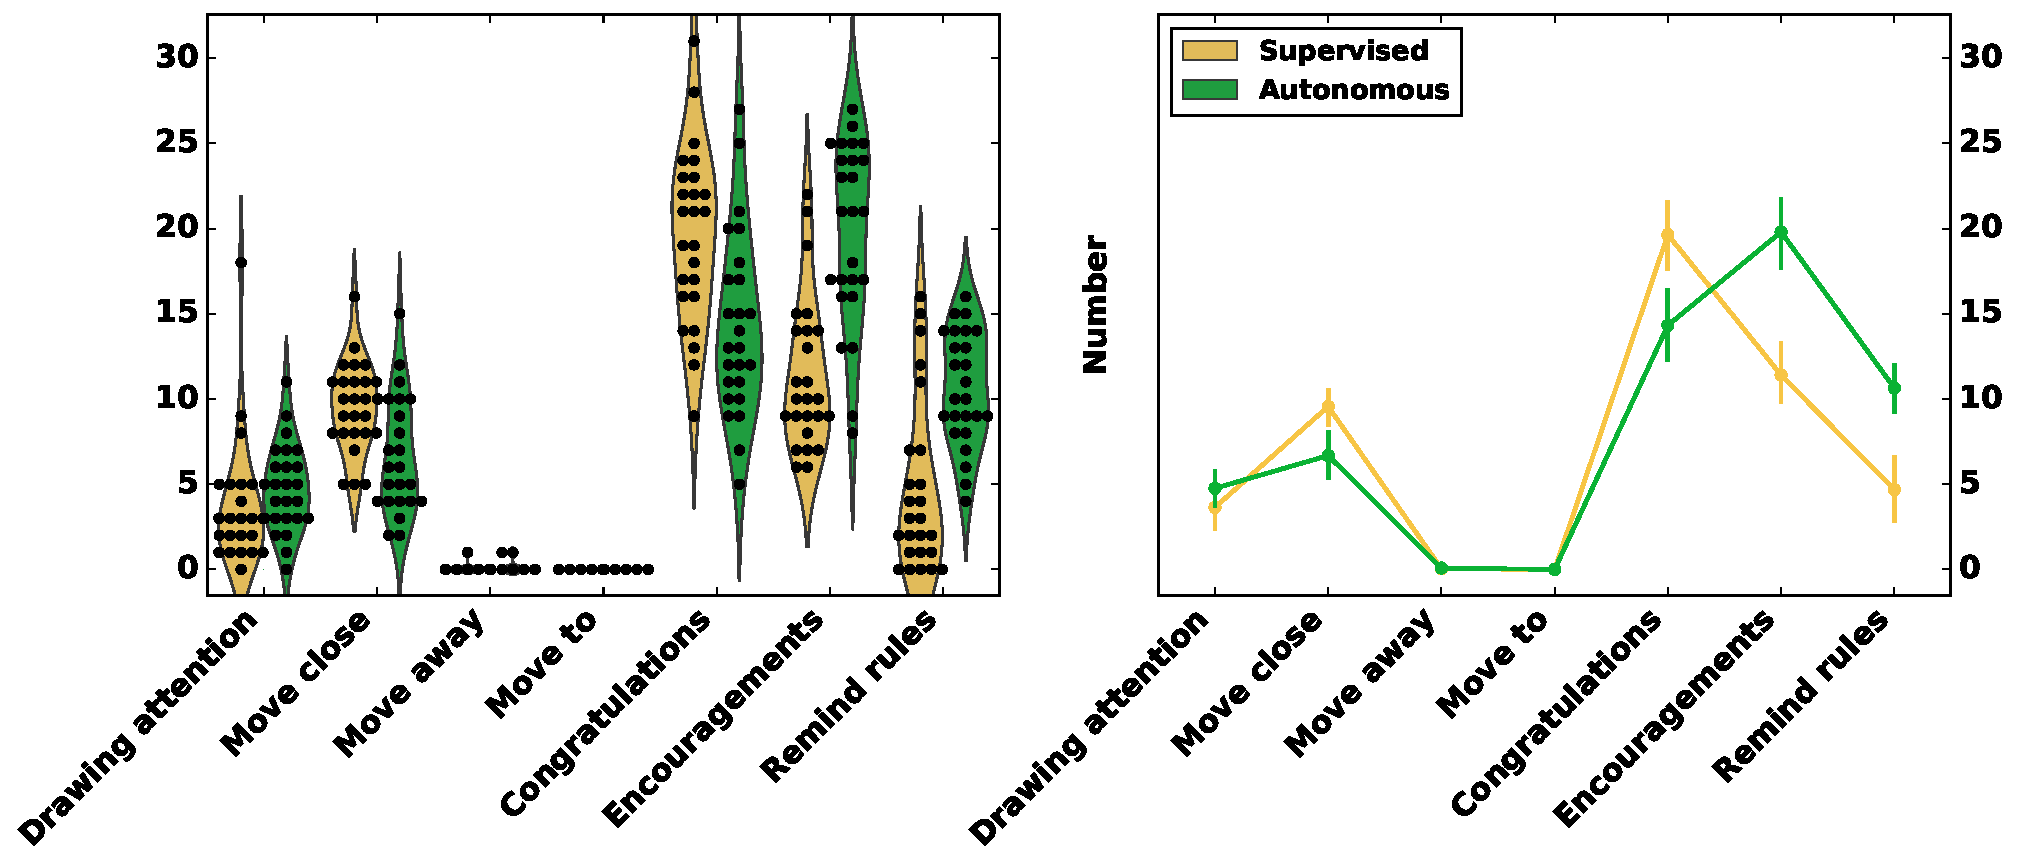
\includegraphics[width=1\linewidth]{actions.pdf}
	\centering
	\caption{Distribution of actions executed by the autonomous and the supervised robot.}
	\label{fig:actions}
\end{figure}

\subsection{Generalisation}
Additionally, providing control to the teacher allows them to specify precisely the desired agent policy. This, combined with the faster learning would allow agents to learn policy tailored to a specific task from a generic definition of the world. This implies that robots could have access to a world definition with a large number of dimensions, allowing for a wide range of policies and task, and from this generic representation of the world, learn a policy directly suited to an application context.

Using guidance from the teacher, the algorithm created an efficient policy mapping a state in 210 dimensions to an action space composed of 655 discrete actions, thus demonstrating that from a large state and action spaces, this type of interaction allows to create a policy tailored to a specific task. Other tasks and policies could have been covered with the same representation of the world, interface and algorithm, but were not evaluated in that study.

\subsection{Trust}
By progressively teaching an agent to behave, a human teacher can build a model of the agent and create expectations on the agent's behaviour. This accumulated knowledge might lead to a trust between the teacher and the learner: by supervising the agent interacting in the world, the teacher can estimate the performance of the displayed policy. This trust and knowledge about the agent's capabilities might then ease its deployment to interact autonomously in the real world.

In a report written by the teacher while she was supervising the robot, she reported: ``robot was often suggest[ing] good things'' and ``[I] Need to trust the robot more''. In later post-study  interviews she reported that she started to trust the robot in the last interactions, even if this trust never reached a level of full trust. 

\section{Challenges}
While giving human teachers control over the learner's actions provides advantages, it also raises challenges in the design of the interaction, the communication between the learner and its teacher, and in the application to specific time sensitive tasks.
    
\subsection{Interface}
The interface between the learner and the human teacher is key when designing and implementing IML applications. To provide enough control on the robot's behaviour and ensure that the behaviour executed is safe for the agent and the surrounding partners, and leads to an efficient policy, the teacher needs to be able to pre-empt any actions about to be executed by the robot before they negatively impact the environment. Additionally, the teacher needs to be able to select any action for the agent to execute. This implies that the interface needs at the same to communicate the robot's intentions, allow the teacher to evaluate them and select actions to be executed if required.

%Include how it can be mitigated
Human-robot interactions rely on the robot displaying appropriate social behaviours, which requires often large set of sensory inputs to interpret human behaviours and actions. For example, in the study, the robot had access to 655 actions. Giving access to the teacher to such a large action space can be challenging. However, depending of the application, ways can be found to enable it. For example, for the study we used a Graphical User Interface (GUI) and we inferred the exact action selected by the teacher from her interaction with a representation of the world on the GUI instead of providing 655 buttons.
\subsection{Human Time}

Providing the robot's intentions to the teacher early enough to allow them to prevent actions to impact the world can be a challenge too, especially as some environments are time-critical. For example, a car driving semi-autonomously and detecting an obstacle requiring emergency breaking might not have the opportunity to wait for an explicit approval from the teacher. On the other an inappropriate emergency breaking is also highly dangerous as it confuse other drivers. Consequently, the timing of actions to ensure human oversight is a serious challenge when designing semi-autonomous agents.

A second challenges lies in the pace of the interaction, today, a large part of the progress in ML relies on large quantity of data. However, when a human in the action loop, gathering data is a slow and tedious process. Even if datapoints arrive at 1Hz, the time required to accumulate the millions of examples required for methods such as Deep Learning \cite{lecun2015deep} can be prohibitive (more than 250 hours). As such, systems relying on single humans to interactively provide demonstrations needs data-efficient algorithms able to make better use of each datapoint.

%Include how it can be mitigated
The first challenge, time for reaction, can be mitigated by having different threshold for actions, and these threshold could also be learned from the teacher. The second point was addressed in the study by requiring the teacher to specify features of the environment she used to select her actions. This additional information provided crucial information allowing the algorithm to make better use of demonstrations, learning a policy from only a limited number of demonstrations.
%In the study, actions proposed by the robot were automatically executed two seconds after being proposed, which put some pressure on the teacher to react in time. In the future, it could be explored how to provide even more control to the teacher, for example on the rate of suggestions from the robot or the delay before autoexecution of an action. This might help the teacher to control the robot with a lower workload, potentially leading to a between experience for both the teacher and the child interacting with the robot.

\subsection{Human Limits}

The last consideration is human limits. People are sensitive to workload and putting them under too much pressure will lead to human errors that will have to be corrected. When using human teacher, their workload needs to be minimised and ways need to be provided to recover from errors. This recovery needs to handle two sides: the learning algorithm needs to be informed about inaccurate demonstrations, and on the other hand, the impact of the erroneous action on the environment needs to be corrected if possible.
%such as providing corrections for a demonstration or removing a datapoint. In addition to error recovery for the learning algorithm, this error recovery needs also to address the real world impact of actions. 
For example, a robot interacting with humans would need to be able to apologise in case of errors in order to maintain the trust surrounding humans have in it and allow the interaction to continue without friction.

%Include how it can be mitigated
In the study, the teacher reported herself making a few errors throughout the teaching process. She had access to a button to remove datapoints from the learning algorithm and thus correct the algorithm side of the error. However we didn't plan for error recovery in case of incorrect robot behaviour as we initially assumed the human behaviour would be constantly correct. In future implement, we will implement ways to recover from erroneous actions on the environment side too (such as apologies).

\section{Discussion}
The position defended in this paper is as follows:
\begin{quote}
    \textbf{When teaching robots to interact, human teachers should not be simply evaluating an autonomous behaviour, but should be able to control precisely the robot behaviour when required.} %PB: this is a very general statement - taken on its own, it could be seen as a statement in support of full WoZ... True True... PB: much better now!
\end{quote}

The robotics and IML communities need to give a more complete role to the teachers, moving away from acting as simple oracles who label datapoints, and towards the incorporation of all facets of social learning, and taking advantage of the unique opportunities that artificial learners offer. More specifically, a learning robot should leverage people's natural skills at teaching humans and animals (transparency of the teaching process, scaffolding of the teacher's feedback/tasks and constant feedback from the learner), while also profiting from the features only available to artificial agents such as perfect memory, absence of tiredness or boredom, but especially the opportunity to control exactly the learner's behaviour. 
%When teaching robots, humans should therefore utilise their skill gained from teaching human without limiting themselves to these techniques or simply act as a proxy for a reward function from a MDP. %PB: not sure what "...to behave similarly to teaching humans..." means...

Providing humans with this control can be a challenging task given the complexity of the problem. However, we contend that the gains outweigh these limitations dramatically compared to autonomous learning, learning from demonstration or retrospective evaluation of the robot's actions. Consequently, we suggest that research in HRI and IML should dedicate more effort towards this goal.
%OR give more recommendations on how this could be done

%\begin{thebibliography}{99}
\bibliographystyle{IEEEtran}
\bibliography{Bib.bib}

%\end{thebibliography}




\end{document}
